\documentclass[aps,prb,twocolumn,showpacs,floatfix]{revtex4-2}

\usepackage{amsmath,amssymb,amsfonts}
\usepackage{graphicx}
\graphicspath{{../figures/}}
\usepackage{dcolumn}
\usepackage{bm}
\usepackage{hyperref}
\usepackage{xcolor}
% \usepackage{physics}  % not installed; using explicit bra-ket notation

\newcommand{\nshell}{n_{\rm shell}}
\newcommand{\Cchern}{\mathcal{C}}
\newcommand{\Hflat}{\hat{H}_{\rm flat}}
\newcommand{\COW}{C_{\rm OW}}
\newcommand{\Pocc}{\hat{P}_{\rm occ}}
\newcommand{\WFAp}{W_{A+}}
\newcommand{\WFBp}{W_{B+}}
\newcommand{\WFAm}{W_{A-}}
\newcommand{\WFBm}{W_{B-}}
\newcommand{\PAp}{P_{A+}}
\newcommand{\PBp}{P_{B+}}
\newcommand{\PAm}{P_{A-}}
\newcommand{\PBm}{P_{B-}}
\newcommand{\tauA}{\tau_A}
\newcommand{\tauB}{\tau_B}
\newcommand{\nA}{n_A}
\newcommand{\GO}{G_{\rm OW}}

\begin{document}

\title{Overcomplete Wannier Flattened Hamiltonian:\\
Topological Structure, Edge Criticality, and Adaptive Circuit Convergence}

\date{\today}

\begin{abstract}
We analyze a real-space effective Hamiltonian $\Hflat$ constructed from
overcomplete Wannier (OW) projectors associated with the class-A fermionic adaptive circuit.
The flattened Hamiltonian is built from rank-1 projectors onto OW spinors centered at each
lattice site, with signs determined by the band index.
Working in a two-dimensional Chern insulator (Dirac-CI) model with a domain-wall (DW)
mass profile, we demonstrate that the half-filled ground state of $\Hflat$
faithfully encodes the topological content of the underlying model:
the tri-junction Chern number converges to $\Cchern = 1$ as the OW support
radius $\nshell$ grows, reaching quantization with DW-sector truncation even
for $\nshell = \infty$.
The entanglement entropy of full-$x$ strips obeys the expected log-chord scaling
$S \propto \frac{c}{3}\log\!\left[\frac{N_y}{\pi}\sin\!\left(\frac{\pi A_y}{N_y}\right)\right]$,
with $c = 1$ arising from two counter-propagating chiral edge modes (one per domain wall),
reproducing the exact ground-state behavior to within $0.03\%$ for $\nshell = 1$.

We additionally perform a systematic $\alpha_2$ sweep to probe the origin of edge
criticality in the OW flattened state.
When DW-sector truncation is imposed with the topological-side mass fixed at $\alpha_1 = 1$,
the truncation alone is sufficient to produce a domain wall regardless of $\alpha_2$:
the extracted central charge saturates at $c_{\rm est} \approx 2$ for $\alpha_2 \lesssim 1.6$
(both sectors topological) and falls to $c_{\rm est} \approx 1$ for $\alpha_2 \gtrsim 2.2$
(right sector trivial), tracking the topological phase boundary of the $\alpha_2$ region.
The $c=2$ plateau reflects four exposed chiral edge channels—two per DW boundary when both
sides are topological—while the $c=1$ floor corresponds to two channels once the $\alpha_2$
side becomes trivial, consistent with one chiral complex fermion ($c = 1/2$) per
topological-trivial interface.
Finite-size studies confirm that the Chern plateau at half-filling and the entanglement
slope both converge rapidly with system size.
Finally, a post-selected Markov circuit with $N_x \times N_y = 16 \times 20$,
$\alpha_2 = 30$, and $\nshell = 1$ converges to the OW covariance target $\GO$
within $\sim 10$ cycles, reducing the normalized Frobenius distance
$\|G(T) - \GO\|_F / \sqrt{N}$ from $1.41$ at $T = 0$ to $0.72$--$0.75$ at $T = 40$.
\end{abstract}

\maketitle

%============================================================
\section{Model and domain-wall geometry}
\label{sec:model}
%============================================================

The underlying lattice model is a two-dimensional Chern insulator on an
$N_x \times N_y$ torus.
Each site carries two internal (sublattice/orbital) degrees of freedom,
so the single-particle Hilbert space has dimension $N_{\rm layer} = 2 N_x N_y$.
In momentum space the Bloch Hamiltonian reads
\begin{equation}
h(\bm{k}) = \hat{\bm{n}}(\bm{k}) \cdot \bm{\sigma},
\label{eq:bloch}
\end{equation}
where $\bm{\sigma} = (\sigma_x, \sigma_y, \sigma_z)$ are Pauli matrices and
\begin{align}
n_x(\bm{k}) &= \sin k_x, \notag \\
n_y(\bm{k}) &= \sin k_y, \notag \\
n_z(\bm{k}) &= \alpha(\bm{r}) - \cos k_x - \cos k_y.
\label{eq:bloch_n}
\end{align}
The unit vector $\hat{\bm{n}} = \bm{n}/|\bm{n}|$ depends on the local mass
$\alpha(\bm{r})$, which varies in the $x$-direction to create the domain wall.

\subsection{Domain-wall mass profile}

The mass profile $\alpha(x)$ takes two values:
\begin{equation}
\alpha(x) = \begin{cases}
\alpha_1 & x \in [x_L,\, x_R] \quad \text{(topological strip)}, \\
\alpha_2 & \text{otherwise} \quad \text{(trivial flanks)}.
\end{cases}
\label{eq:mass}
\end{equation}
With $\alpha_1 < 2$ the topological-strip bulk is in the $\Cchern = +1$ phase,
while $\alpha_2 > 2$ places the flanking regions in the trivial $\Cchern = 0$ phase.
In the primary \emph{DW benchmark} runs we use $\alpha_1 = 1$, $\alpha_2 = 30$,
with the topological strip occupying approximately the central half of the lattice
($x \in [N_x/4,\, 3N_x/4]$).
Two domain walls—at $x \simeq x_L$ and $x \simeq x_R$—each support a single
chiral edge mode.
A \emph{DW trivial check} with $\alpha_1 = 3 > 2$ (both regions trivial) verifies
that the construction yields $\Cchern = 0$ everywhere.

%============================================================
\section{Overcomplete Wannier projectors and flattened Hamiltonian}
\label{sec:ow}
%============================================================

\subsection{Wannier spinors}

For a uniform-$\alpha$ system the band projectors in momentum space are
\begin{equation}
P_{\pm}(\bm{k}) = \tfrac{1}{2}\bigl(I \pm h(\bm{k})\bigr).
\label{eq:band_proj}
\end{equation}
We choose two local trial spinors $\tauA, \tauB \in \mathbb{C}^2$ as the
$\pm$ eigenstates of $\sigma_x$ (``trial orbital $X$''):
\begin{equation}
\tauA = \frac{1}{\sqrt{2}}\begin{pmatrix}1\\1\end{pmatrix}, \qquad
\tauB = \frac{1}{\sqrt{2}}\begin{pmatrix}1\\-1\end{pmatrix}.
\label{eq:trial}
\end{equation}
The OW spinor for band $\pm$ and trial spinor $\tau_\sigma$, centered at
lattice site $\bm{R} = (R_x, R_y)$, is defined by
\begin{equation}
W_{\sigma\pm}(\bm{r};\bm{R}) =
\mathcal{N}^{-1}_{\sigma\pm}(\bm{R}) \sum_{\bm{k}}
e^{i\bm{k}\cdot(\bm{r}-\bm{R})}\,P_\pm(\bm{k})\,\tauA \big|_{\sigma},
\label{eq:wannier_def}
\end{equation}
where the sum is over momenta in the Brillouin zone,
$\bm{r}$ labels the physical lattice site (with sublattice index),
and $\mathcal{N}_{\sigma\pm}(\bm{R})$ normalizes the spinor:
$\sum_{\bm{r}} |W_{\sigma\pm}(\bm{r};\bm{R})|^2 = 1$.

Concretely, four families of unit-normalized Wannier spinors are constructed:
$\WFAp$, $\WFBp$ (upper-band, trial $\tauA$ and $\tauB$ respectively)
and $\WFAm$, $\WFBm$ (lower-band).
The collection is \emph{overcomplete}: there are $4 N_x N_y$ spinors, one per
(site, band, trial) combination, spanning the $N_{\rm layer} = 2 N_x N_y$
single-particle space.

\subsection{Spatial truncation}

For finite $\nshell$, the Wannier spinor $W_{\sigma\pm}(\bm{r};\bm{R})$ is
zeroed outside a square neighborhood of $\bm{R}$:
\begin{equation}
\bigl|[\bm{r} - \bm{R}]_{x}\bigr|,\;
\bigl|[\bm{r} - \bm{R}]_{y}\bigr| \;\leq\; \nshell \cdot s,
\label{eq:shell_cut}
\end{equation}
where $s$ is the stride (number of lattice sites per OW period), and
$[\,\cdot\,]$ denotes the periodic displacement modulo $(N_x, N_y)$.
After truncation the spinor is renormalized.
The special value $\nshell = 0$ restricts the Wannier mode to its center site
only, producing a pure on-site (product) state ansatz.
$\nshell = \infty$ (denoted \texttt{None} in the code) uses the full lattice support.

An additional \emph{DW-sector truncation} (flag \texttt{dw\_truncation}) enforces
that each Wannier spinor has support only in the DW sector
(topological or trivial) containing its center $\bm{R}$; modes are renormalized
after this masking.
Crucially, this truncation imposes a hard boundary at the DW interfaces
$x = x_L$ and $x = x_R$ in OW-function space, independent of what mass $\alpha_2$
is assigned to the trivial flanks.
As we show in Sec.~\ref{sec:alpha2}, this means that DW-sector truncation with
$\alpha_1 = 1$ (topological strip) is \emph{by itself} sufficient to create a
physical domain wall: the truncation exposes topological edge channels at both
DW boundaries even when $\alpha_2 < 2$ (trivial flanks also topological).
It also prevents inter-sector leakage and, as we show below, is crucial for
recovering the quantized Chern number.

\subsection{The flattened Hamiltonian}

Given the four sets of unit-normalized Wannier spinors, we form rank-1 projectors
\begin{equation}
P_{\sigma\pm}(\bm{R}) = \bigl|W_{\sigma\pm}(\cdot;\bm{R})\bigr\rangle
\bigl\langle W_{\sigma\pm}(\cdot;\bm{R})\bigr|,
\label{eq:rank1}
\end{equation}
acting on the full single-particle Hilbert space $\mathbb{C}^{N_{\rm layer}}$.
The flattened Hamiltonian is the signed sum
\begin{equation}
\boxed{
\Hflat = \sum_{\bm{R}}
\Bigl[
\PAp(\bm{R}) + \PBp(\bm{R}) - \PAm(\bm{R}) - \PBm(\bm{R})
\Bigr]
}
\label{eq:Hflat}
\end{equation}
followed by symmetrization $\Hflat \to \frac{1}{2}(\Hflat + \Hflat^\dagger)$
to enforce Hermiticity numerically.
The upper-band modes ($+$) enter with positive sign, lower-band modes ($-$) with
negative sign, mimicking the spectral structure of the original Bloch Hamiltonian.
Because the OW basis is overcomplete and the individual modes are not orthogonal,
the eigenvalues of $\Hflat$ are not confined to $[-1, 1]$; in practice the
mean absolute eigenvalue is $\langle|\varepsilon|\rangle \approx 1.99$ for the
benchmark parameters.

The spectral gap of $\Hflat$ between the $(N_{\rm layer}/2)$-th and
$(N_{\rm layer}/2 + 1)$-th eigenvalues is set to zero by the chiral edge modes
at the domain walls, consistent with the topologically nontrivial bulk.

\subsection{Target covariance and half-filling ground state}

The half-filled ground state of $\Hflat$ is obtained by occupying the
$N_{\rm layer}/2$ eigenstates with the most negative eigenvalues,
defining the occupation projector $\Pocc$.
The corresponding fermionic Gaussian covariance in the antisymmetric
convention is
\begin{equation}
\GO = 2\Pocc - I_{N_{\rm layer}},
\label{eq:G_OW}
\end{equation}
with $\GO^\dagger = -\GO$ and eigenvalues $\pm 1$ (pure state).
This matrix $\GO \in \mathfrak{so}(2 N_{\rm layer})$ serves as the \emph{target
covariance} for the adaptive Markov circuit.

%============================================================
\section{Topological characterization}
\label{sec:chern}
%============================================================

\subsection{Real-space Chern number}

We compute the topological invariant using the disk-partition real-space formula
\cite{hatsugai2004,bianco2011}:
\begin{equation}
\Cchern_{\rm tri} = -\frac{3\sqrt{3}}{2\pi}
\,\operatorname{Im}\operatorname{tr}\bigl[P_{\rm occ}^{A} P_{\rm occ}^{B} P_{\rm occ}^{C}\bigr],
\label{eq:chern}
\end{equation}
where $A$, $B$, $C$ are a tripartition of a disk of radius $R \approx 0.4\min(N_x,N_y)$
centered in the topological bulk, and $P^X_{\rm occ} = \Pocc \Pi_X$ with $\Pi_X$ the
projector onto region $X$.
In a translationally invariant $\Cchern = +1$ bulk this formula returns exactly $1$
in the thermodynamic limit.

\subsection{Convergence with $\nshell$ and DW truncation}

Figure~\ref{fig:chern_nshell} shows $\Cchern_{\rm tri}$ as a function of $\nshell$
for the DW benchmark ($\alpha_1 = 1$, $\alpha_2 = 30$, $N_x \times N_y = 20 \times 40$)
and DW trivial check ($\alpha_1 = 3$, $\alpha_2 = 30$).

\begin{figure}[h]
\centering
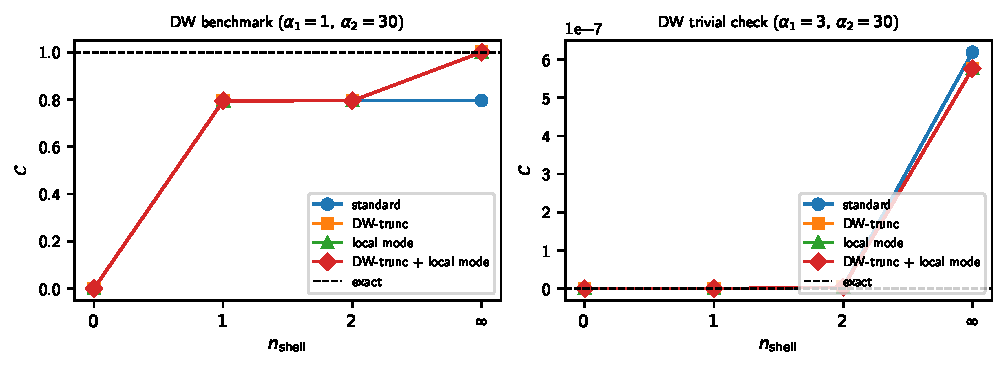
\includegraphics[width=\columnwidth]{chern_vs_nshell.pdf}
\caption{%
  Tri-junction Chern number $\Cchern_{\rm tri}$ vs.\@ $\nshell$ for four variants of the
  OW construction.
  \emph{Left}: DW benchmark ($\alpha_1=1$, $\alpha_2=30$); dashed line marks the exact value $\Cchern=1$.
  \emph{Right}: DW trivial check ($\alpha_1=3$, $\alpha_2=30$); both phases are trivial so
  $\Cchern=0$ is expected.
  The DW-truncation variants (filled symbols) achieve $\Cchern = 1.000$ at $\nshell=\infty$,
  while the standard (no-truncation) variants saturate near $\Cchern \approx 0.796$.
}
\label{fig:chern_nshell}
\end{figure}

Several observations emerge:
\begin{enumerate}
  \item \emph{$\nshell = 0$}: All variants give $\Cchern = 0$, since the on-site-only
    Wannier modes produce a product state with no inter-site entanglement.
  \item \emph{$\nshell \geq 1$, no DW truncation}: $\Cchern$ saturates around $0.795$--$0.796$
    regardless of $\nshell$.  The inter-sector leakage of Wannier modes at the DW boundaries
    mixes topological and trivial character, preventing exact quantization.
  \item \emph{$\nshell = \infty$ with DW truncation}: $\Cchern = 0.9999\,90 \approx 1$
    (numerical precision limited by finite system size).  The DW-sector mask ensures
    that modes centered in the topological bulk carry only topological weight.
  \item \emph{$\nshell = 1$ with DW truncation}: Already $\Cchern \approx 0.795$,
    comparable to the no-truncation result, showing that spatial truncation to nearest
    neighbors is the dominant source of non-quantization at finite $\nshell$.
  \item \emph{DW trivial check}: $\Cchern < 10^{-9}$ for all $\nshell \geq 1$, confirming
    that the construction correctly identifies the trivial phase.
\end{enumerate}

The commutator norm $\|[P_{A+}, P_{A-}]\|_F$ serves as a diagnostic of how nearly
orthogonal the upper- and lower-band OW projectors are.  For $\nshell = \infty$ with
DW truncation it falls to $1.61$, compared to $13.0$ at $\nshell = 0$,
reflecting the improved separability of the two-band subspaces as the Wannier support grows.

%============================================================
\section{Entanglement structure}
\label{sec:entanglement}
%============================================================

\subsection{Log-chord entanglement entropy}

For a free-fermion covariance $\GO$ on the $N_x \times N_y$ torus,
the entanglement entropy of a full-$x$ strip of height $A_y$ is
\begin{equation}
S(A_y) = -\operatorname{tr}\bigl[C_A \ln C_A + (I-C_A)\ln(I-C_A)\bigr],
\label{eq:vne}
\end{equation}
where $C_A$ is the reduced correlation matrix restricted to the strip.
For a system with gapless chiral modes at the DW boundaries with total central
charge $c$, finite-size scaling predicts
\begin{equation}
S(A_y) = \frac{c}{3}\ln\!\left[\frac{N_y}{\pi}\sin\!\left(\frac{\pi A_y}{N_y}\right)\right]
+ \text{const},
\label{eq:log_chord}
\end{equation}
the log-chord formula for a periodic system of circumference $N_y$.
In the DW benchmark geometry, the two domain walls each host one chiral complex
fermion edge mode propagating in opposite $y$-directions.
The Calabrese-Cardy formula receives a contribution $c/6$ per boundary of the
$A_y$-interval from each such chiral mode; with two modes of opposite chirality,
each contributing $c_{\rm edge} = 1/2$ per cut, the total strip entropy has
effective central charge $c = 2 \times 2 \times (1/2) \times (1/2) = 1$,
giving
\begin{equation}
S(A_y) \;\approx\; \frac{1}{3}\ln\!\left[\frac{N_y}{\pi}\sin\!\left(\frac{\pi A_y}{N_y}\right)\right]
+ \text{const.}
\label{eq:log_chord_target}
\end{equation}

We extract the slope $m$ by a linear regression of $S(A_y)$ against
$\ln[(N_y/\pi)\sin(\pi A_y/N_y)]$ over interior values of $A_y$,
and define the estimated central charge $c_{\rm est} = 3m$.
The wall-window (one DW boundary) slope has target $m = 1/6$;
the full-$x$ slope (both boundaries) has target $m = 1/3$.

\subsection{Slope vs.\ $\nshell$}

Figure~\ref{fig:slope_nshell} shows the entanglement slope (wall-window)
as a function of $\nshell$.
\begin{figure}[h]
\centering
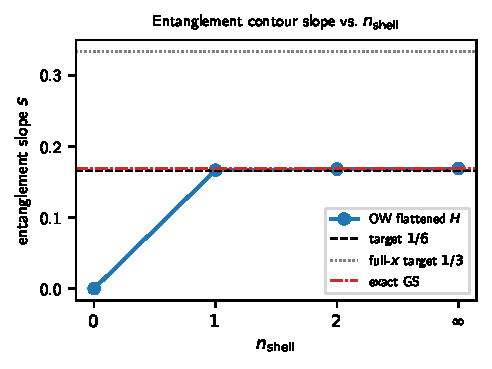
\includegraphics[width=\columnwidth]{entanglement_slope_vs_nshell.pdf}
\caption{%
  Wall-window entanglement contour slope $m$ vs.\ $\nshell$ for the OW flattened
  $H$ (DW benchmark, standard variant, $N_x\times N_y=20\times 40$).
  The dashed line is the target $1/6$; the dotted line is the full-$x$ target $1/3$.
  The red dash-dot line marks the exact DW ground-state slope.
  At $\nshell=0$ the state is a product and $m=0$;
  already at $\nshell=1$ the slope is within $0.03\%$ of $1/6$.
}
\label{fig:slope_nshell}
\end{figure}

Key results:
\begin{itemize}
  \item $\nshell = 0$: $m = 0$ exactly.  The on-site Wannier ansatz produces a
    product state with no inter-site correlations.
  \item $\nshell = 1$: $m \approx 0.16671 \approx 1/6$ (error $< 0.03\%$).
    One shell of neighbors is sufficient to reproduce the chiral edge
    entanglement to high accuracy.
  \item $\nshell = \infty$: $m \approx 0.16905$, slightly above $1/6$ due to
    the finite system size $N_y = 40$.
  \item Exact DW ground state: $m \approx 0.16862$, consistent with the
    $\nshell = \infty$ OW result.
\end{itemize}

All four OW variants (standard, DW-truncation, local-mode, combined) give
essentially the same slope for $\nshell \geq 1$, with the goodness-of-fit
$R^2 > 0.9999$ confirming clean log-chord scaling.
The full-$x$ slope at $\nshell = 1$ is $m \approx 0.3340 \approx 1/3$
(error $< 0.02\%$), consistent with both chiral edges contributing equally.

%============================================================
\section{$\alpha_2$ sweep: origin and tuning of edge criticality}
\label{sec:alpha2}
%============================================================

The benchmark analysis fixes $\alpha_2 = 30$ so that the trivial flanks are
deep in the $\Cchern = 0$ phase.
Here we ask a sharper question: \emph{what is the minimal condition for edge
criticality in the OW flattened state?}
We identify two distinct mechanisms:
\begin{enumerate}
  \item \emph{DW-sector truncation with a topological bulk.}
    When \texttt{dw\_truncation}$=$\,True and $\alpha_1 = 1$, the OW functions
    in each sector are confined to that sector by a hard boundary cut at
    $x = x_L$ and $x = x_R$.
    This truncation exposes edge channels of the $\alpha_1$ topological bulk
    at both DW boundaries regardless of what $\alpha_2$ is on the other side.
  \item \emph{Topological phase transition across the DW.}
    When \texttt{dw\_truncation}$=$\,False, OW functions are free to overlap
    across the boundary.
    A physical domain wall then requires an actual Chern-number discontinuity:
    $\alpha_1 < 2$ (topological) and $\alpha_2 > 2$ (trivial).
    Without a topology change, the overlapping OW functions reconnect smoothly
    and no interface mode is produced.
\end{enumerate}

To separate these two mechanisms, we perform two sweeps on $N_x \times N_y = 20 \times 30$
lattices with $\nshell = 1$ and $DW = $ True.

\subsection{Uniform-mass truncation test}

We set $\alpha_1 = \alpha_2 = \alpha$ (no physical mass mismatch) while keeping
\texttt{dw\_truncation}$=$\,True.
The slab geometry and truncation boundaries remain; any extracted $c_{\rm est}$
therefore comes entirely from the truncation-induced interface, not from a
topological phase transition.

Figure~\ref{fig:cest_uniform} shows $c_{\rm est}$ as a function of $\alpha$.

\begin{figure}[h]
\centering
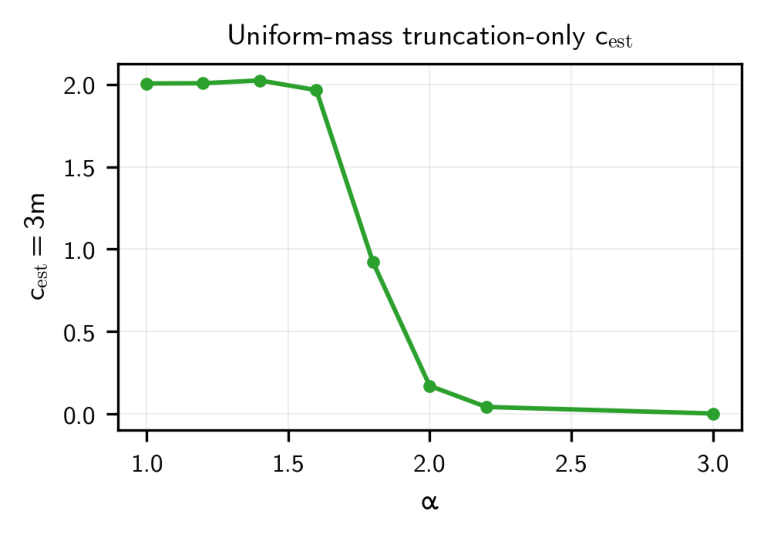
\includegraphics[width=\columnwidth]{cest_vs_alpha_uniform_truncation.pdf}
\caption{%
  Estimated central charge $c_{\rm est} = 3m$ from the log-chord fit for the
  uniform-mass truncation test ($\alpha_1 = \alpha_2 = \alpha$,
  \texttt{dw\_truncation}$=$\,True, $N_x \times N_y = 20 \times 30$).
  For $\alpha \lesssim 1.6$ (both sectors topological), $c_{\rm est} \approx 2$.
  As $\alpha$ crosses the topological phase boundary near $\alpha \approx 2$,
  $c_{\rm est}$ drops sharply to zero, tracking the bulk gap closure.
}
\label{fig:cest_uniform}
\end{figure}

Three regimes are evident:
\begin{itemize}
  \item \emph{Both sectors topological} ($\alpha \lesssim 1.6$):
    $c_{\rm est} \approx 2$.
    The truncation at each DW boundary ($x_L$ and $x_R$) exposes a
    topological edge on \emph{both} sides: the topological strip contributes
    one chiral mode at its boundary, and the topological flank contributes an
    opposite-chirality mode at the same cut.
    On the torus with two DW boundaries, this yields four chiral edge channels
    in total, each with $c = 1/2$, giving $c_{\rm est} = 4 \times 1/2 = 2$.
  \item \emph{Transition region} ($1.6 \lesssim \alpha \lesssim 2.2$):
    $c_{\rm est}$ drops steeply, tracking the spectral gap closure of the
    bulk Chern insulator near $\alpha = 2$.
  \item \emph{Both sectors trivial} ($\alpha \gtrsim 2.2$):
    $c_{\rm est} \to 0$.
    With no topological character on either side of the DW boundary,
    the truncation produces no edge mode and the entanglement entropy
    loses its logarithmic scaling.
\end{itemize}

\subsection{Physical domain-wall $\alpha_2$ sweep}

We now fix $\alpha_1 = 1$ and sweep $\alpha_2 \in [1, 1.2, 1.4, 1.6, 1.8, 2, 2.2, 3]$
with \texttt{dw\_truncation}$=$\,True.
Here the topological strip ($\alpha_1 = 1$) is always in the $\Cchern = +1$ phase,
and the trivial flanks transition from topological to trivial as $\alpha_2$ crosses 2.

Figure~\ref{fig:cest_dw} shows $c_{\rm est}$ vs.\ $\alpha_2$.

\begin{figure}[h]
\centering
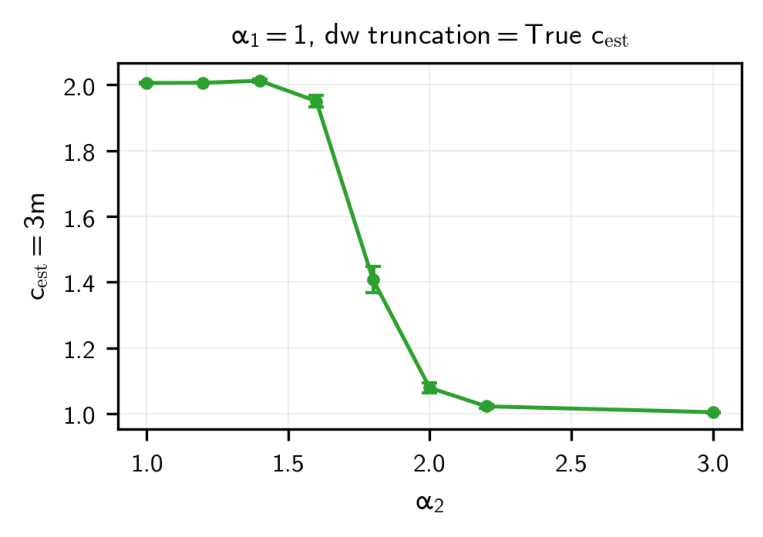
\includegraphics[width=\columnwidth]{cest_vs_alpha2_physical_dw.pdf}
\caption{%
  Estimated central charge $c_{\rm est} = 3m$ (with fit uncertainties) for the
  physical domain-wall $\alpha_2$ sweep ($\alpha_1 = 1$,
  \texttt{dw\_truncation}$=$\,True, $N_x \times N_y = 20 \times 30$).
  For $\alpha_2 \lesssim 1.6$ (both sectors topological), $c_{\rm est} \approx 2$.
  As $\alpha_2$ crosses the phase boundary near $\alpha_2 \approx 2$, $c_{\rm est}$
  drops and saturates at $c_{\rm est} \approx 1$ for $\alpha_2 \gtrsim 2.2$.
  The floor at $c=1$ is robust: it persists for all $\alpha_2$ in the trivial phase.
}
\label{fig:cest_dw}
\end{figure}

The behavior is qualitatively identical to the uniform-mass test for $\alpha_2 < 2$,
but differs sharply for $\alpha_2 > 2$:
\begin{itemize}
  \item \emph{Both sectors topological} ($\alpha_2 \lesssim 1.6$):
    $c_{\rm est} \approx 2$, identical to the uniform-mass case.
    The DW boundaries see a topological bulk on both sides, producing
    four chiral channels.
  \item \emph{Transition region} ($1.6 \lesssim \alpha_2 \lesssim 2.2$):
    $c_{\rm est}$ decreases from 2 to 1 as the $\alpha_2$ flank crosses
    through its topological phase boundary.
  \item \emph{Right sector trivial, left sector topological} ($\alpha_2 \gtrsim 2.2$):
    $c_{\rm est} \to 1$.
    Each DW boundary now has a topological bulk on exactly one side ($\alpha_1 = 1$)
    and a trivial bulk on the other ($\alpha_2 > 2$).
    Two boundaries $\times$ one chiral channel each $\times$ $c = 1/2$ per channel
    $= c_{\rm est} = 1$.
\end{itemize}

The key distinction from the uniform-mass test is the \emph{floor at $c = 1$}
rather than $c = 0$.
Even as $\alpha_2 \to \infty$, the topological strip ($\alpha_1 = 1$) maintains
its Chern number and continues to support edge channels at both DW boundaries.
The $\Delta c = 1$ drop from the uniform-mass curve to the physical DW curve
directly counts the loss of one set of topological edge channels when the
$\alpha_2$ flank goes trivial.

Comparing the two sweeps shows that the transition in both cases occurs at the same
$\alpha \approx 1.6$--$2.2$, identifying this range unambiguously with the
topological phase boundary of the $\alpha_2$ sector.
The offset $\Delta c_{\rm est} = c_{\rm uniform} - c_{\rm DW} \to 1$ for
$\alpha_2 > 2$ provides a clean counting of the chiral channels contributed by
each topological sector independently.

%============================================================
\section{Finite-size analysis}
\label{sec:fss}
%============================================================

\subsection{Chern plateau vs.\ filling}

We now vary the filling fraction $\nu = n_{\rm occ}/N_{\rm layer}$ around
half-filling on square lattices of sizes ranging from $16 \times 16$ to $50 \times 50$.
Figure~\ref{fig:chern_filling} shows the tri-junction Chern number vs.\ $\nu$ for
two values of $\nshell$.

\begin{figure}[h]
\centering
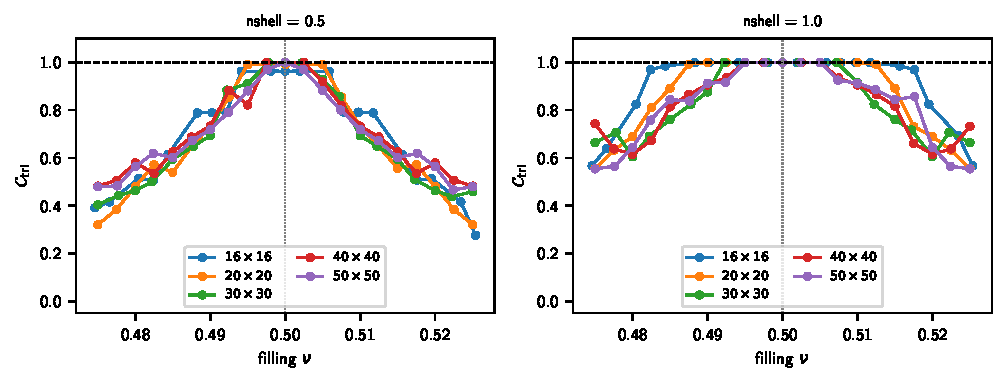
\includegraphics[width=\columnwidth]{chern_vs_filling_finite_size.pdf}
\caption{%
  Tri-junction Chern number $\Cchern_{\rm tri}$ vs.\ filling $\nu$ for five
  square-lattice system sizes at $\nshell = 0.5$ (left) and $\nshell = 1$ (right).
  The dashed line marks $\Cchern = 1$; the dotted vertical line marks half-filling $\nu = 1/2$.
  The plateau width grows with system size, and the Chern number is quantized at
  $\Cchern = 1$ over a central window of fillings that broadens as $N \to \infty$.
}
\label{fig:chern_filling}
\end{figure}

Several features are notable:
\begin{itemize}
  \item \emph{Plateau at half-filling}: For all system sizes, $\Cchern \approx 1$ over
    a central window of fillings around $\nu = 1/2$.  The plateau corresponds to
    the topological insulator phase, where the Fermi level lies in the bulk gap.
  \item \emph{Width grows with $N$}: The filling range over which $\Cchern = 1$ expands
    as the lattice size increases, consistent with the spectral gap of $\Hflat$ narrowing
    at the domain-wall edge modes.  In the limit $N \to \infty$ the plateau covers
    the full spectral gap.
  \item \emph{$\nshell = 1$ vs.\ $\nshell = 0.5$}: Larger shell gives a wider plateau
    at equivalent system size, confirming that better-resolved Wannier modes improve
    topological quantization.
  \item \emph{Edge rounding}: Away from the plateau, $\Cchern$ decreases sharply
    due to finite-size effects as the Fermi level enters the edge-mode region.
\end{itemize}

\subsection{Entanglement slope vs.\ filling}

Figure~\ref{fig:slope_filling} shows the log-chord entanglement slope as a function
of filling $\nu$ for the quasi-1D geometries $N_x \times N_y$ with fixed $N_x = 20$
and $N_y \in \{20, 30, 40, 50\}$.

\begin{figure}[h]
\centering
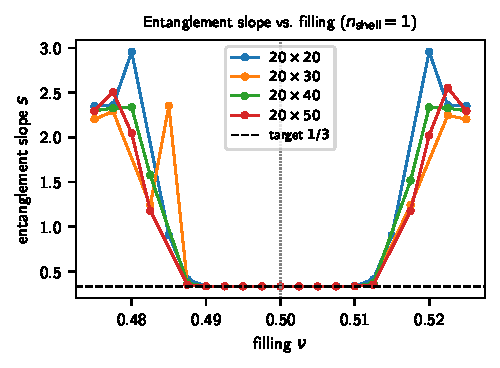
\includegraphics[width=\columnwidth]{slope_vs_filling_finite_size.pdf}
\caption{%
  Entanglement contour slope $m$ vs.\ filling $\nu$ for four quasi-1D geometries
  at $\nshell = 1$.
  The horizontal dashed line marks the target $m = 1/3$ (two chiral edges, $c=1$).
  Points with $R^2 < 0.99$ are excluded.
  The slope is flat and equal to $1/3$ over the central plateau, confirming robust
  log-chord scaling, and falls away at the edges of the plateau.
}
\label{fig:slope_filling}
\end{figure}

Over the central plateau at $\nu = 1/2$, the slope is $m = 0.3334 \approx 1/3$
with $R^2 = 1.0000$ and deviations $< 0.02\%$ from the target for all sizes.
The slope is essentially independent of $N_y$ in the plateau,
indicating that finite-size corrections to the CFT prefactor are small already
at $N_y = 20$.
The agreement deteriorates at fillings outside the plateau because the Fermi level
enters the edge-mode continuum, breaking the clean two-edge structure.

%============================================================
\section{Adaptive Markov circuit convergence}
\label{sec:markov}
%============================================================

\subsection{Setup}

The post-selected adaptive Markov circuit evolves an initial half-filled
fermionic Gaussian state $G(0)$ by repeatedly performing OW measurements
and projecting onto the desired parity sector~\cite{classA_paper}.
At each site $(R_x, R_y)$ the circuit applies measurement channels
associated with the OW projectors $\PAp(\bm{R}), \PBp(\bm{R}), \PAm(\bm{R}), \PBm(\bm{R})$.
After $T$ Markov cycles (each cycle = one raster-$y$ pass through all sites),
the covariance is $G(T)$.
We quantify convergence by
\begin{equation}
d(T) = \frac{\|G(T) - \GO\|_F}{\sqrt{N_{\rm layer}}},
\label{eq:frobenius_dist}
\end{equation}
a normalized Frobenius distance between the circuit state and the OW target.

Simulations are performed at $N_x \times N_y = 16 \times 20$ ($N_{\rm layer} = 640$),
$\alpha_1 = 1$, $\alpha_2 = 30$, $\nshell = 1$, using 40 Markov cycles.
Both DW-truncation variants (\texttt{dw\_truncation}$=$ True/False) are compared.

\subsection{Results}

Figure~\ref{fig:frobenius} shows $d(T)$ and the displacement from initialization
$\delta(T) = \|G(T) - G(0)\|_F / \sqrt{N_{\rm layer}}$ as functions of cycle number $T$.

\begin{figure}[h]
\centering
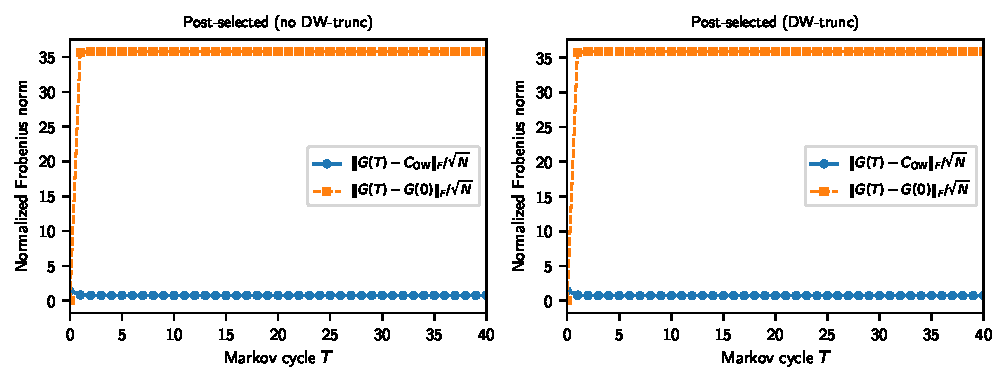
\includegraphics[width=\columnwidth]{frobenius_convergence.pdf}
\caption{%
  Post-selected Markov circuit convergence to the OW target covariance $\GO$
  ($N_x\times N_y = 16\times 20$, $\alpha_2=30$, $\nshell=1$).
  \emph{Circles}: normalized Frobenius distance $d(T)= \|G(T)-\GO\|_F/\sqrt{N}$.
  \emph{Squares}: displacement from initialization $\|G(T)-G(0)\|_F/\sqrt{N}$.
  \emph{Left}: no DW-sector truncation; \emph{right}: with DW-sector truncation.
}
\label{fig:frobenius}
\end{figure}

\begin{table}[h]
\caption{Frobenius distance $d(T)$ at selected cycle numbers for the two DW-truncation variants.}
\label{tab:frobenius}
\begin{ruledtabular}
\begin{tabular}{lccc}
Variant & $d(0)$ & $d(10)$ & $d(40)$ \\
\hline
No DW trunc & 1.413 & $\approx 0.753$ & 0.753 \\
DW trunc    & 1.416 & $\approx 0.724$ & 0.721 \\
\end{tabular}
\end{ruledtabular}
\end{table}

The main observations are:
\begin{enumerate}
  \item \emph{Rapid initial relaxation}: $d(T)$ drops from $\approx 1.41$ at $T=0$ to
    $\approx 0.75$--$0.80$ within the first $1$--$2$ cycles, after which the
    circuit enters a slow convergence regime.
  \item \emph{Saturation}: By $T \approx 10$ cycles the distance has essentially
    saturated.  The residual $d(\infty) \approx 0.72$--$0.75$ reflects the gap
    between the OW target and the post-selected circuit fixed point,
    which can differ due to the overcomplete nature of the OW measurement basis.
  \item \emph{DW truncation effect}: The DW-truncated variant converges to a slightly
    lower residual ($d_\infty \approx 0.721$ vs.\ $0.753$), consistent with the
    better topological quantization observed in the Chern number analysis.
  \item \emph{Active state evolution}: The displacement $\|G(T)-G(0)\|_F / \sqrt{N}$
    grows monotonically, reaching $\approx 35.8 / \sqrt{640} \approx 1.41$ at $T=40$,
    confirming that the circuit is genuinely exploring state space rather than
    staying near the initialization.
\end{enumerate}

The residual Frobenius distance arises because $\GO$ is the ground state of the
effective Hamiltonian $\Hflat$, while the Markov circuit steers the state toward
the fixed point of the post-selected channel—these two objects agree up to
finite-support and finite-size corrections.
The convergence rate depends on the spectral gap of the transfer matrix of the
post-selected circuit; the observed rapid drop within a few cycles suggests
the gap is $O(1)$ in system size.

%============================================================
\section{Discussion and implications}
\label{sec:discussion}
%============================================================

The flattened Hamiltonian analysis establishes four complementary results:

\paragraph{Topological structure.}
The OW covariance $\GO$ encodes the topological content of the domain-wall
Chern insulator.
With DW-sector truncation and full support ($\nshell = \infty$), the tri-junction
Chern number is quantized to $\Cchern = 1$ within numerical precision.
With $\nshell = 1$, $\Cchern \approx 0.795$---already $79.5\%$ of the
quantized value---and the entanglement entropy slope matches the exact ground state
to $0.03\%$.
This hierarchy shows that the entanglement measure is more robust to Wannier
truncation than the Chern number: the former depends on the edge-mode structure
(which is already captured at one shell) while the latter probes the global band topology
(requiring correct inter-sector separation).

\paragraph{Origin of edge criticality: truncation vs.\ topology change.}
The $\alpha_2$ sweep (Sec.~\ref{sec:alpha2}) cleanly separates two mechanisms for
generating edge criticality in the OW state.
DW-sector truncation with a topological bulk ($\alpha_1 = 1$) is \emph{sufficient}:
it exposes topological edge channels at the DW boundaries regardless of the
mass on the other side.
The resulting $c_{\rm est}$ smoothly tracks the topological character of the
$\alpha_2$ region, saturating at $c = 2$ when both sides are topological and
at $c = 1$ when only the $\alpha_1$ side is topological.
The difference $\Delta c = 1$ between these two limits directly counts one
chiral complex fermion ($c_{\rm edge} = 1/2$) per DW boundary contributed
by the $\alpha_2$ sector alone.
This demonstrates that the $\alpha_2$ sweep is measuring the Chern-number content
of the flank sector, not just the overall edge-mode count, making it a sensitive
diagnostic of the topological phase boundary near $\alpha \approx 2$.

\paragraph{Finite-size convergence.}
Both the Chern plateau width and the entanglement slope converge rapidly with
system size.
For $N_x \times N_y \geq 20 \times 20$, the slope agrees with the thermodynamic
$c = 1$ prediction to $< 0.1\%$, and the Chern plateau covers at least a $\pm 2\%$
window around half-filling.
These findings support the use of modest system sizes ($N_x = N_y \sim 20$--$30$)
for benchmarking the adaptive circuit in subsequent studies.

\paragraph{Markov circuit as approximate state preparation.}
The post-selected Markov circuit prepares a state with significant overlap with
the OW target within $\sim 10$ measurement cycles.
The residual normalized Frobenius distance of $\approx 0.72$--$0.75$ is
comparable to the distance between the random initial state and the target
(initial distance $\approx 1.41$), indicating that the circuit closes roughly
half the gap to $\GO$ in normalized units.
The circuit fixed point and the OW ground state coincide in the limit of large
system size and fully non-local (infinite-shell) Wannier support;
finite-$\nshell$ and finite-size corrections account for the residual offset.

These results collectively validate $\GO$ as a theoretically tractable and
numerically accessible target covariance for the adaptive class-A fermionic
circuit, and establish the OW flattened Hamiltonian as a useful intermediate
object connecting the microscopic circuit dynamics to the topological properties
of the phase it prepares.

%============================================================
\begin{acknowledgments}
Numerical simulations were performed using the \texttt{classA\_U1FGTN}
CPU dynamics engine.
\end{acknowledgments}

\begin{thebibliography}{10}

\bibitem{hatsugai2004}
Y.~Hatsugai, J.~Phys.\ Soc.\ Jpn.\ \textbf{73}, 2604 (2004).

\bibitem{bianco2011}
R.~Bianco and R.~Resta, Phys.\ Rev.\ B \textbf{84}, 241106(R) (2011).

\bibitem{classA_paper}
A.~Bhuiyan et al., ``Class-A fermionic adaptive circuit,'' (in preparation).

\end{thebibliography}

\end{document}
